\documentclass[conference]{IEEEtran}
\IEEEoverridecommandlockouts

% ── Encoding & font ──────────────────────────────────────────────────────────
\usepackage[utf8]{inputenc}
\usepackage[T1]{fontenc}

% ── Core IEEE packages ────────────────────────────────────────────────────────
\usepackage{cite}
\usepackage{amsmath,amssymb,amsfonts}
\usepackage{graphicx}
\usepackage{textcomp}
\usepackage{xcolor}

% ── Additional packages ───────────────────────────────────────────────────────
\usepackage{booktabs}          % professional table rules
\usepackage{caption}           % caption* for unnumbered captions

% ── Graphics paths (relative to this file) ───────────────────────────────────
\graphicspath{{../output/figures/}{figures/}}

\def\BibTeX{{\rm B\kern-.05em{\sc i\kern-.025em b}\kern-.08em
    T\kern-.1667em\lower.7ex\hbox{E}\kern-.125emX}}

% ── Convenience macros ────────────────────────────────────────────────────────
\newcommand{\qreal}{Q_{\mathrm{real}}}
\newcommand{\qvirt}{Q_{\mathrm{virtual}}}
\newcommand{\pacb}{p_{\mathrm{acb}}}
\newcommand{\ema}{\mathrm{EMA}}
\newcommand{\lam}{\lambda}

% =============================================================================
\begin{document}
% =============================================================================

\title{5G RRC Signaling Storm Mitigation via a Proactive Digital Twin Architecture with Continuous Calibration}

\author{%
\IEEEauthorblockN{1\textsuperscript{st} Ömer Dikyol}
\IEEEauthorblockA{\textit{Department of Computer Engineering}\\
\textit{Istanbul Technical University}\\
Istanbul, Turkey\\
dikyol25@itu.edu.tr}
}

\maketitle

% =============================================================================
% ABSTRACT
% =============================================================================
\begin{abstract}
The Random Access Channel (RACH) infrastructure in the 5G New Radio (NR) architecture has a structural vulnerability to high volume RRC signaling storm traffic generated by targeted botnet attacks. The current Access Class Barring (ACB) mechanism suffers from control loop latency, as the decision to throttle traffic is made only after buffer saturation, making it ineffective when load is already rising. Predictive Digital Twin (DT) based approaches can mitigate this latency. However, model drift under non stationary traffic conditions causes cumulative growth in state mirroring error and degrades prediction quality. This paper proposes a proactive Digital Twin architecture with a continuous calibration loop that actively suppresses model drift. A two state Continuous Time Markov Chain (CTMC) based MMPP/M/c/K queue is used to model the physical gNB RACH, and proactive control decisions are derived from an Exponential Moving Average (EMA) predictor. Monte Carlo experiments conducted over 1000 seconds with $N=10$ independent random seeds show that the calibration loop reduces state mirroring error by 42\% compared to an uncalibrated DT. The connection success rate is statistically equivalent to the reactive baseline; P90 and P99 queueing delay values are reduced.
\end{abstract}

\begin{IEEEkeywords}
5G NR, RRC Signaling Storm, Digital Twin, Access Class Barring, MMPP/M/c/K, Exponential Moving Average, Model Drift, State Mirroring Error, Queueing Delay
\end{IEEEkeywords}

% =============================================================================
% SECTION 1: INTRODUCTION
% =============================================================================
\section{Introduction}

The 5G New Radio (NR) architecture positions the Radio Resource Control (RRC) protocol as a central resource management layer to support increasing user density and diversified service requirements. The gNodeB (gNB) processes RRC connection requests from user devices through the Random Access Channel (RACH) and responds through a limited number of preamble channels. While this design provides effective resource allocation under normal traffic conditions, it contains a major security weakness against coordinated botnet attacks.

Botnet traffic generates high volume, bursty waves of RRC connection requests over short intervals and intentionally saturates the RACH buffer. Such attacks are referred to in the literature as an \emph{RRC Signaling Storm}~\cite{b1} and lead to depletion of gNB resources, causing legitimate user requests to be rejected. Given that 5G NR is expected to support applications requiring low latency and high reliability, such as autonomous vehicles, remote surgery, and industrial automation, these disruptions can result in critical Quality of Service (QoS) failures.

The Access Class Barring (ACB) mechanism defined in 3GPP standards is the primary reactive tool for limiting RACH load. However, this mechanism suffers from a fundamental \emph{Control Loop Latency} problem: the throttling decision can be made only after buffer saturation has already been observed, which makes the mechanism ineffective during the very period when the load increase should have been prevented~\cite{b2}.

To address this limitation, predictive control approaches have attracted growing interest. The Digital Twin (DT) paradigm enables continuous maintenance of a virtual copy of the physical system and allows inferences from that copy to shape control decisions~\cite{b3}. Nevertheless, standard DT based predictors are vulnerable to \emph{Model Drift} under non stationary burst conditions. The deviation between the state representations of the physical system and its virtual copy, namely the \emph{State Mirroring Error}, accumulates over time and weakens proactive control.

This work proposes a \emph{Calibrated Digital Twin} architecture with a continuous calibration loop to close this gap. The main contributions of the paper are as follows:

\begin{enumerate}
\item \textbf{Realistic traffic model:} A two state MMPP/M/c/K queue is designed to model 5G RRC signaling storm conditions, and the burst dynamics of adversarial traffic are captured through a Continuous Time Markov Chain (CTMC).
\item \textbf{Continuous calibration loop:} A calibration mechanism is introduced that updates the Exponential Moving Average (EMA) weight with an asymmetric step rule when the state mirroring error exceeds a threshold. This mechanism reduces state mirroring error by 42\%.
\item \textbf{Proactive QoS improvement:} The effects of the calibration loop on $P_{success}$ and the queueing delay distribution are evaluated through Monte Carlo experiments with $N=10$ independent seeds.
\item \textbf{Epsilon sensitivity analysis:} The impact of the calibration trigger threshold $\varepsilon$ on system performance is examined through an exploratory single seed sweep, showing that $\varepsilon = 40$ achieves the highest composite objective in that run while $\varepsilon = 10$ remains a conservative default just above the normal traffic noise floor.
\end{enumerate}

% =============================================================================
% SECTION 2: RELATED WORK
% =============================================================================
\section{Related Work}

\subsection{Reactive Methods and Their Limitations}

The most common reactive mechanism for preventing RACH overload is the Access Class Barring (ACB) method defined in 3GPP TS 38.331~\cite{b4}. The original ACB framework introduced in LTE Release 11 relied on a binary barring mechanism that grouped devices by access class (AC 0 to 9). The gNB broadcast a barring factor $p$ and a barring duration $T_{acb}$ through System Information Block 2 (SIB2), causing devices in selected access classes to defer their RACH transmissions probabilistically.

With 5G NR Release 15, 3GPP adopted the more flexible \emph{Unified Access Control} (UAC) framework~\cite{b4}. UAC provides a two dimensional policy table that cross maps traffic categories and access identities. The barring factors are broadcast to all devices via the uac-BarringInfo field in System Information Block 1 (SIB1). The $\pacb$ value computed by the proposed DT controller at each $\Delta$ step maps directly to this UAC barring factor. The DT is therefore designed to inject $\pacb$ into the SIB1 broadcast of the gNB and provides a standards compliant real time control interface. This allows the proposed proactive controller to be integrated into existing 3GPP signaling without requiring protocol changes.

This general mechanism has been studied extensively in both LTE and 5G NR, and adaptive ACB variants that adjust barring parameters based on queue occupancy have been proposed~\cite{b5}.

However, all reactive ACB and UAC variants remain subject to a basic causality constraint: the barring decision depends on observing the queue length, processing that observation, and delivering the control signal through SIB1. This inevitably creates control loop latency. Seo \emph{et al.}~\cite{b6} showed that random access delay requirements can be violated when the access procedure approaches unstable or saturated operating regions, confirming the practical inadequacy of purely reactive control loops.

\subsection{Proactive and Predictive Approaches}

In response to the limitations of reactive methods, proactive control approaches have been developed to predict future traffic conditions and apply throttling policies in advance. Approaches in this area include Markov decision processes~\cite{b7}, deep learning based resource allocation~\cite{b8}, and time series based load prediction~\cite{b9}.

The Digital Twin paradigm offers a broader framework in which the virtual representation of the physical system is updated continuously through real time feedback~\cite{b10}. The broader 5G and cyber physical systems literature has explored network digital twins~\cite{b11}, network slicing security~\cite{b12}, and DT based anomaly detection~\cite{b13}. However, most existing DT based network controllers do not update their predictive behavior during runtime. In botnet driven RRC signaling storm scenarios, this leads to model drift and growing state mirroring error. The proposed calibrated DT architecture addresses this specific gap.

% =============================================================================
% SECTION 3: SYSTEM MODEL
% =============================================================================
\section{System Model}

\subsection{Network Environment and Attack Scenario}

The scenario targets a single gNB cell operating under the 5G NR framework. The botnet generates high density, bursty RRC connection requests designed to saturate the physical gNB buffer through the RACH. Performance is evaluated against a reactive baseline.

\subsection{Traffic Model: MMPP/M/c/K Queue}

To model abrupt transitions in adversarial traffic, a two state CTMC based Markov Modulated Poisson Process (MMPP) is adopted. The system is denoted as $MMPP/M/c/K$: the arrival process is MMPP, service times are exponentially distributed, there are $c$ parallel servers, and the total capacity is limited to $K$.

The CTMC has two states. In $S_0$ (normal state), legitimate RRC connection requests arrive at rate $\lambda_{\mathrm{low}} = 10$ requests/s. In $S_1$ (burst state), adversarial botnet traffic arrives at rate $\lambda_{\mathrm{high}} = 500$ requests/s. Transitions between the two states are defined by the generator matrix $Q$:

\begin{equation}
Q = \begin{bmatrix}
    -\alpha_{mmpp} & \alpha_{mmpp} \\
    \beta_{mmpp}   & -\beta_{mmpp}
\end{bmatrix}
\label{eq:generator}
\end{equation}

where $\alpha_{mmpp} = 0.1\ \mathrm{s}^{-1}$ is the transition rate from $S_0$ to $S_1$, and $\beta_{mmpp} = 0.5\ \mathrm{s}^{-1}$ is the transition rate from $S_1$ to $S_0$. The state sojourn time in state $i$ is sampled from $\mathrm{Exp}(|Q_{ii}|)$. This reproduces CTMC dynamics exactly in a discrete event simulation environment without requiring matrix exponential calculations.

\subsection{Physical gNB Constraints}

The physical gNB RACH contains $c = 54$ preamble channels. The total system capacity is limited to $K = 200$. The instantaneous queue length, $\qreal$, is defined as the total number of requests in service and in waiting. Requests arriving when $\qreal(t) \geq K$ are dropped immediately because of buffer overflow.

% =============================================================================
% SECTION 4: PROPOSED METHOD
% =============================================================================
\section{Proposed Method}

\subsection{Proactive Digital Twin Architecture}

The proposed method consists of a proactive Digital Twin controller running in parallel with the physical gNB. The DT executes a unified pipeline with control interval $\Delta = 1\ \mathrm{s}$ and three sequential stages: observation and prediction, control decision, and continuous calibration.

\subsection{EMA Based Arrival Rate Prediction}

The DT predicts the future arrival rate using an Exponential Moving Average (EMA) filter:

\begin{equation}
\ema_t = \alpha \cdot \lambda_{\mathrm{current}} + (1 - \alpha) \cdot \ema_{t-1}
\label{eq:ema}
\end{equation}

where $\lambda_{\mathrm{current}} = n_{\mathrm{window}}/\Delta$, $n_{\mathrm{window}}$ is the number of arrivals observed during the interval $\Delta$, and $\alpha \in [0,1]$ is the dynamic correction weight. The initial value is set to $\alpha_0 = 0.2$, chosen empirically and confirmed to produce stable EMA estimates under normal traffic conditions prior to calibration loop activation.

\subsection{Stochastic Control Policy: $\pacb$ Computation}

The DT analytically computes the minimum dropping probability required to prevent $\qreal$ from exceeding $K$ during the next control step:

\begin{equation}
\pacb = \max\!\left(0,\ \min\!\left(1,\ 1 - \frac{K - \qreal}
    {\max(\ema_t \cdot \Delta,\ \varepsilon_g)}\right)\right)
\label{eq:pacb}
\end{equation}

where $\varepsilon_g = 10^{-9}$ protects against division by zero. The value $\pacb$ is applied as an independent Bernoulli trial to each incoming request and forms a stochastic barring mechanism compatible with the Unified Access Control framework in 3GPP TS 38.331.

\subsection{Virtual Queue Update}

To internally emulate the controlled physical system, the DT maintains a virtual queue $\qvirt$:

\begin{equation}
\begin{aligned}
\qvirt(t{+}\Delta) = \mathrm{clip}\!\big(&
    \qvirt(t) + \ema_t (1 - \pacb)\Delta - c\Delta,\\
    &0,\; K\big)
\end{aligned}
\label{eq:qvirtual}
\end{equation}

The $(1 - \pacb)$ factor is mathematically necessary. Once the control policy is applied, the actual amount of traffic entering the system is $\ema_t \cdot (1 - \pacb) \cdot \Delta$, not $\ema_t \cdot \Delta$. Omitting this factor causes $\qvirt$ to converge artificially toward $K$ during burst periods, which inflates the state mirroring error and triggers calibration incorrectly.

\subsection{State Mirroring Error}

The instantaneous deviation between the DT and the physical system is measured by the state mirroring error $E$:

\begin{equation}
E(t) = \left| \qreal(t) - \qvirt(t) \right|
\label{eq:error}
\end{equation}

\subsection{Continuous Calibration Loop}

After $E$ is computed at each $\Delta$ step, the DT updates the weight $\alpha$ using an asymmetric step rule:

\begin{equation}
\alpha \leftarrow \begin{cases}
    \min(\alpha_{max},\ \alpha + \delta^{+}) & \text{if } E > \varepsilon \\
    \max(\alpha_{min},\ \alpha - \delta^{-}) & \text{otherwise}
\end{cases}
\label{eq:calibration}
\end{equation}

In this work, $\varepsilon = 10$, $\delta^{+} = 0.05$, $\delta^{-} = 0.01$, $\alpha_{min} = 0.05$, and $\alpha_{max} = 1.0$. The deliberate asymmetry reflects two distinct operational requirements. The rapid increase through $\delta^{+}$ at the onset of an attack transforms the EMA filter into a high frequency structure and quickly reduces the influence of outdated observations. When traffic returns to normal, the small decay step $\delta^{-}$ preserves statistical stability.

\subsection{Unified Control Loop}

All components above are combined in the unified control loop given in Algorithm 1. The loop is triggered every $\Delta$ seconds, consumes only $\qreal$ and $n_{\mathrm{win}}$ as inputs, and produces $\pacb$, the updated $\qvirt$, and the updated $\alpha$ as outputs.

\begin{figure}[t]
\vspace{-2pt}
\noindent\rule{\columnwidth}{0.5pt}\\[-5pt]
\noindent\rule{\columnwidth}{0.15pt}
\vspace{3pt}
{\small
\noindent\textbf{Algorithm 1:} Calibrated Digital Twin Control Loop\\[4pt]
\noindent\textbf{Input:} $\qreal$,\ $n_{\mathrm{win}}$,\ $\Delta$,\ $\varepsilon$,\ $\alpha$,\ $\alpha_{min}$,\ $\alpha_{max}$,\ $\delta^{+}$,\ $\delta^{-}$\\
\noindent\textbf{Output:} $\pacb$, updated $\qvirt$, updated $\alpha$\\[4pt]
\noindent\textbf{Every} $\Delta$ step:\\[2pt]
\noindent\phantom{0}1:\enspace $\lambda_{cur} \leftarrow n_{\mathrm{win}} / \Delta$ \hfill\textit{current arrival rate}\\
\noindent\phantom{0}2:\enspace $\ema_t \leftarrow \alpha\cdot\lambda_{cur}+(1-\alpha)\cdot\ema_{t-1}$ \hfill\textit{EMA update}\\
\noindent\phantom{0}3:\enspace $d \leftarrow \max\!\left(\ema_t\cdot\Delta,\ 10^{-9}\right)$\\
\noindent\phantom{0}4:\enspace $\pacb \leftarrow \max\!\left(0,\,\min\!\left(1,\,1-(K-\qreal)/d\right)\right)$ \hfill\textit{Eq. \eqref{eq:pacb}}\\
\noindent\phantom{0}5:\enspace $\qvirt \leftarrow \mathrm{clip}\!\left(\qvirt+\ema_t(1{-}\pacb)\Delta-c\Delta,\;0,\;K\right)$ \hfill\textit{Eq. \eqref{eq:qvirtual}}\\
\noindent\phantom{0}6:\enspace $E \leftarrow \left|\qreal - \qvirt\right|$ \hfill\textit{Eq. \eqref{eq:error}}\\
\noindent\phantom{0}7:\enspace \textbf{if} $E > \varepsilon$ \textbf{then}\\
\noindent\phantom{07:}\enspace $\alpha \leftarrow \min(\alpha_{max},\;\alpha + \delta^{+})$ \hfill\textit{fast adaptation}\\
\noindent\phantom{0}8:\enspace \textbf{else}\\
\noindent\phantom{08:}\enspace $\alpha \leftarrow \max(\alpha_{min},\;\alpha - \delta^{-})$ \hfill\textit{slow decay}\\
\noindent\phantom{0}9:\enspace \textbf{end if} \hfill\textit{Eq. \eqref{eq:calibration}}\\
\noindent10:\enspace $\text{drop\_rate} \leftarrow \pacb$ \hfill\textit{actuate control decision to gNB}
}
\vspace{3pt}
\noindent\rule{\columnwidth}{0.15pt}\\[-5pt]
\noindent\rule{\columnwidth}{0.5pt}
\end{figure}

% =============================================================================
% SECTION 5: PERFORMANCE EVALUATION
% =============================================================================
\section{Performance Evaluation}

\subsection{Simulation Parameters}

Monte Carlo experiments were run over $T_{\mathrm{sim}} = 1000\ \mathrm{s}$ with $N = 10$ independent random seeds. The simulation was implemented as a discrete event system using SimPy in Python 3.10 and analyzed with NumPy and Pandas. The main parameters are summarized in Table~\ref{tab:params}.

\begin{table}[t]
\caption{Simulation Parameters}
\label{tab:params}
\begin{center}
\begin{tabular}{lll}
\toprule
\textbf{Parameter} & \textbf{Symbol} & \textbf{Value} \\
\midrule
Total time                  & $T_{\mathrm{sim}}$ & 1000 s \\
RACH preamble channels      & $c$                & 54 \\
Buffer capacity             & $K$                & 200 \\
Normal arrival rate         & $\lambda_{low}$   & 10 requests/s \\
Burst arrival rate          & $\lambda_{high}$  & 500 requests/s \\
Normal$\to$Burst transition & $\alpha_{mmpp}$   & 0.1 s$^{-1}$ \\
Burst$\to$Normal transition & $\beta_{mmpp}$    & 0.5 s$^{-1}$ \\
Control interval            & $\Delta$          & 1 s \\
Calibration threshold       & $\varepsilon$     & 10 \\
Initial EMA weight          & $\alpha_0$        & 0.20 \\
Reactive threshold          & $0.8K$             & 160 \\
Reactive drop rate          & ---                & 0.50 \\
\bottomrule
\end{tabular}
\end{center}
\end{table}

\subsection{State Mirroring Error Analysis}

Table~\ref{tab:metrics} summarizes the main performance metrics of the three methods across $N=10$ seeds. Confidence intervals are computed using $\bar{x} \pm 1.96 \cdot \hat{\sigma}/\sqrt{N}$.

\begin{table}[t]
\caption{Multi Seed Performance Metrics ($N=10$,\ $T_{\mathrm{sim}}=1000$~s)}
\label{tab:metrics}
\begin{center}
\scriptsize
\setlength{\tabcolsep}{3pt}
\begin{tabular}{lccc}
\toprule
\textbf{Method} & $P_{success}$ & $P_{drop}$ & $E_{mean}$ \\
\textbf{} & ($\pm$ 95\% CI) & ($\pm$ 95\% CI) & ($\pm$ 95\% CI) \\
\midrule
Reactive Baseline   & $0.310 \pm 0.015$ & $0.688 \pm 0.015$ & $0.00 \pm 0.00$ \\
DT (No Calibration) & $0.301 \pm 0.011$ & $0.698 \pm 0.011$ & $85.03 \pm 4.40$ \\
Calibrated DT       & $0.309 \pm 0.019$ & $0.690 \pm 0.019$ & $49.14 \pm 3.09$ \\
\bottomrule
\end{tabular}
\end{center}
\end{table}

The state mirroring error analysis confirms the primary finding of the calibration mechanism. The uncalibrated DT has $E_{mean} = 85.03$. Once the continuous calibration loop is activated, $E_{mean}$ drops to $49.14$, which corresponds to a \textbf{42\% reduction} relative to the uncalibrated DT. Figure~\ref{fig:E_ci} shows the state mirroring error time series with 95\% confidence interval bands.

\begin{figure}[t]
\centerline{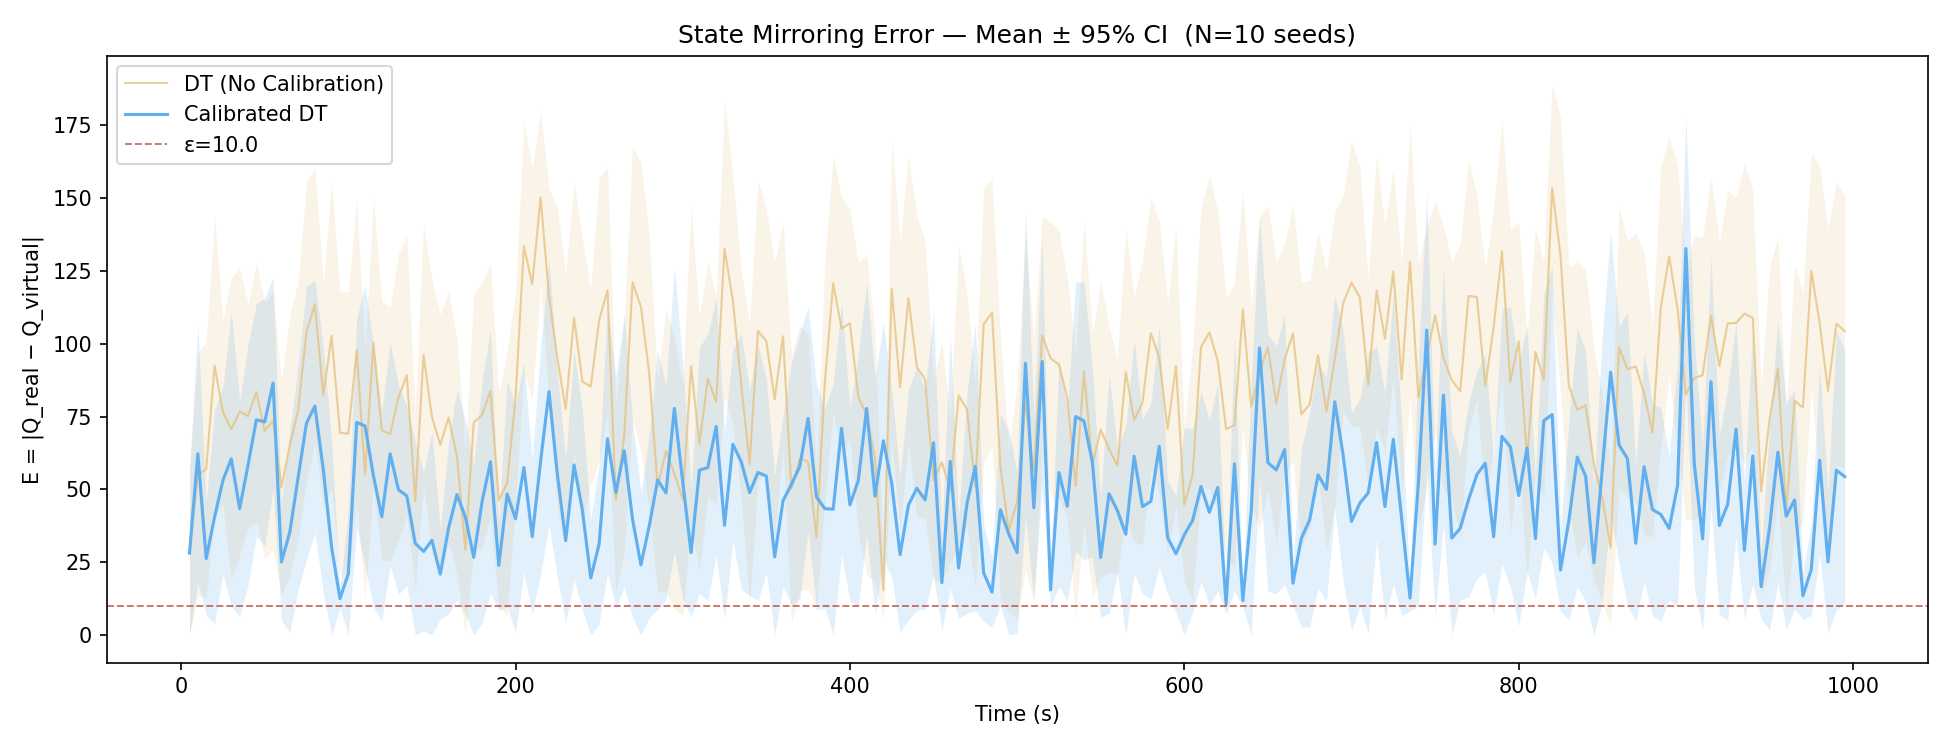
\includegraphics[width=\columnwidth]{phase5_E_ci.png}}
\caption{State mirroring error time series comparing Calibrated DT and DT without calibration. Shaded regions indicate the 95\% confidence interval across $N=10$ seeds. The horizontal dashed line represents the calibration threshold $\varepsilon=10$.}
\label{fig:E_ci}
\end{figure}

\subsection{Connection Performance and Queue Stability}

In terms of connection success, the observed ordering is Reactive Baseline ($P_{success} = 0.310$), Calibrated DT ($P_{success} = 0.309$), and DT without calibration ($P_{success} = 0.301$). The difference between the reactive baseline and the calibrated DT (0.001) is not statistically meaningful because the confidence intervals overlap substantially. However, this numerical similarity should not be read as mechanistic equivalence.

The reactive baseline reaches a similar $P_{success}$ only after the queue approaches saturation, that is, after the threshold $\qreal > 0.8K$ is exceeded and the dropping policy activates. The calibrated DT instead increases $\pacb$ gradually before $\qreal$ reaches $K$, thereby keeping the queue length in a more stable region. Figure~\ref{fig:q_real_ci} presents the queue stability comparison.

\begin{figure}[t]
\centerline{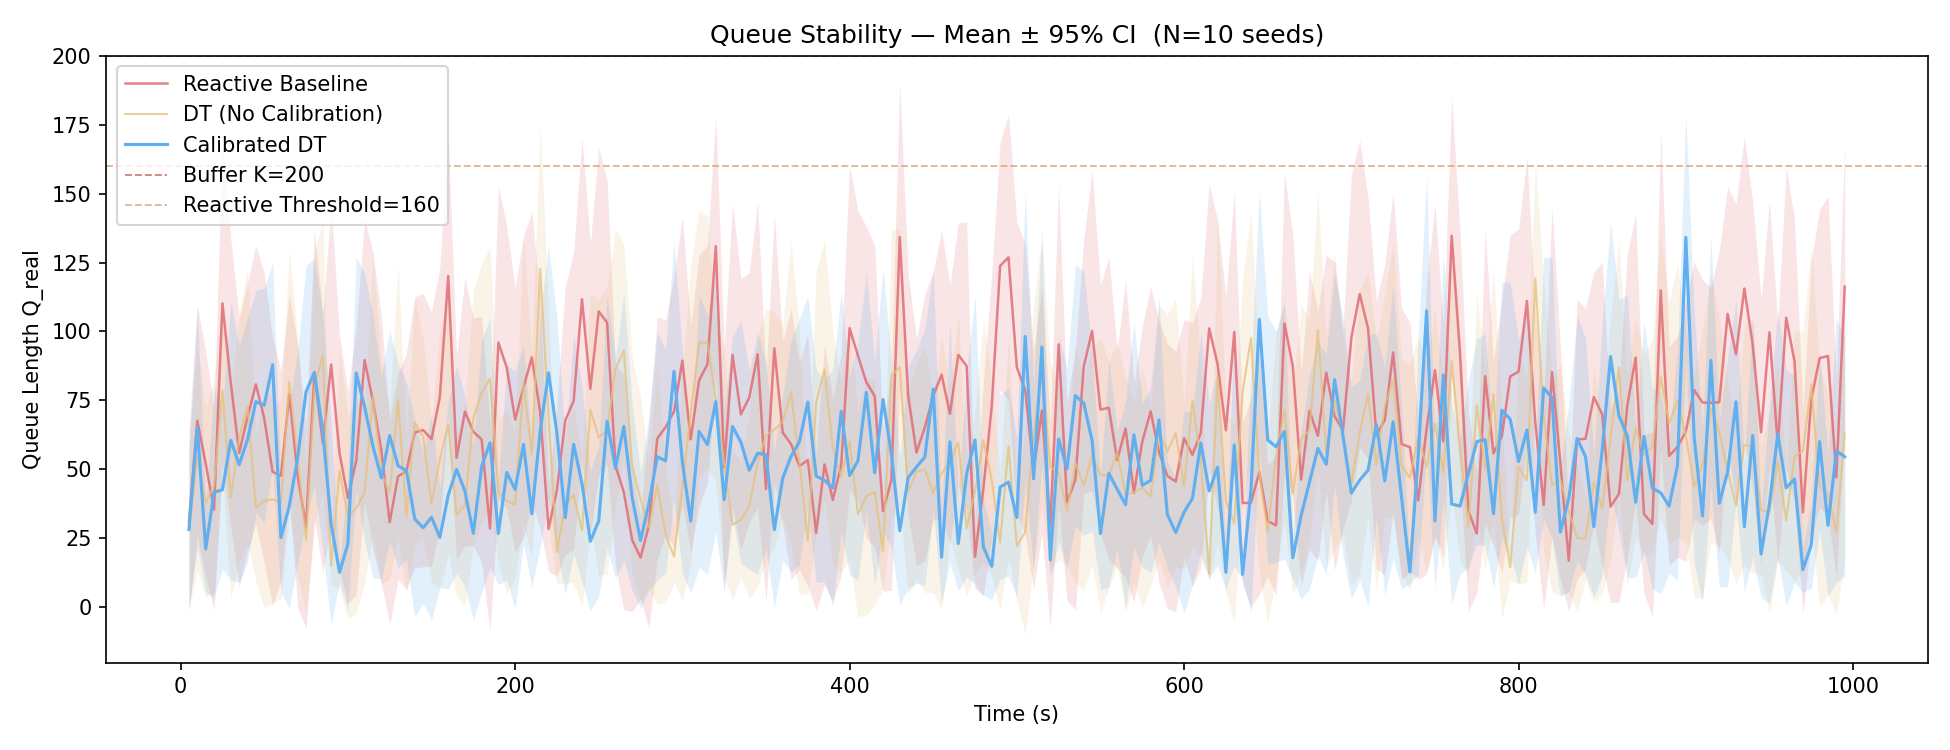
\includegraphics[width=\columnwidth]{phase5_q_real_ci.png}}
\caption{Queue length $\qreal$ time series comparing the three methods with 95\% confidence interval bands. The upper dashed line denotes the buffer limit $K=200$, and the lower dashed line denotes the reactive threshold $0.8K=160$.}
\label{fig:q_real_ci}
\end{figure}

\subsection{Queueing Delay: Cumulative Distribution Function Analysis}

The advantage of the calibrated DT becomes clearer in the per request queueing delay distribution. The Cumulative Distribution Function (CDF) in Figure~\ref{fig:delay_cdf} is built by pooling delay values from all served requests across $N=10$ seeds.

\begin{figure}[t]
\centerline{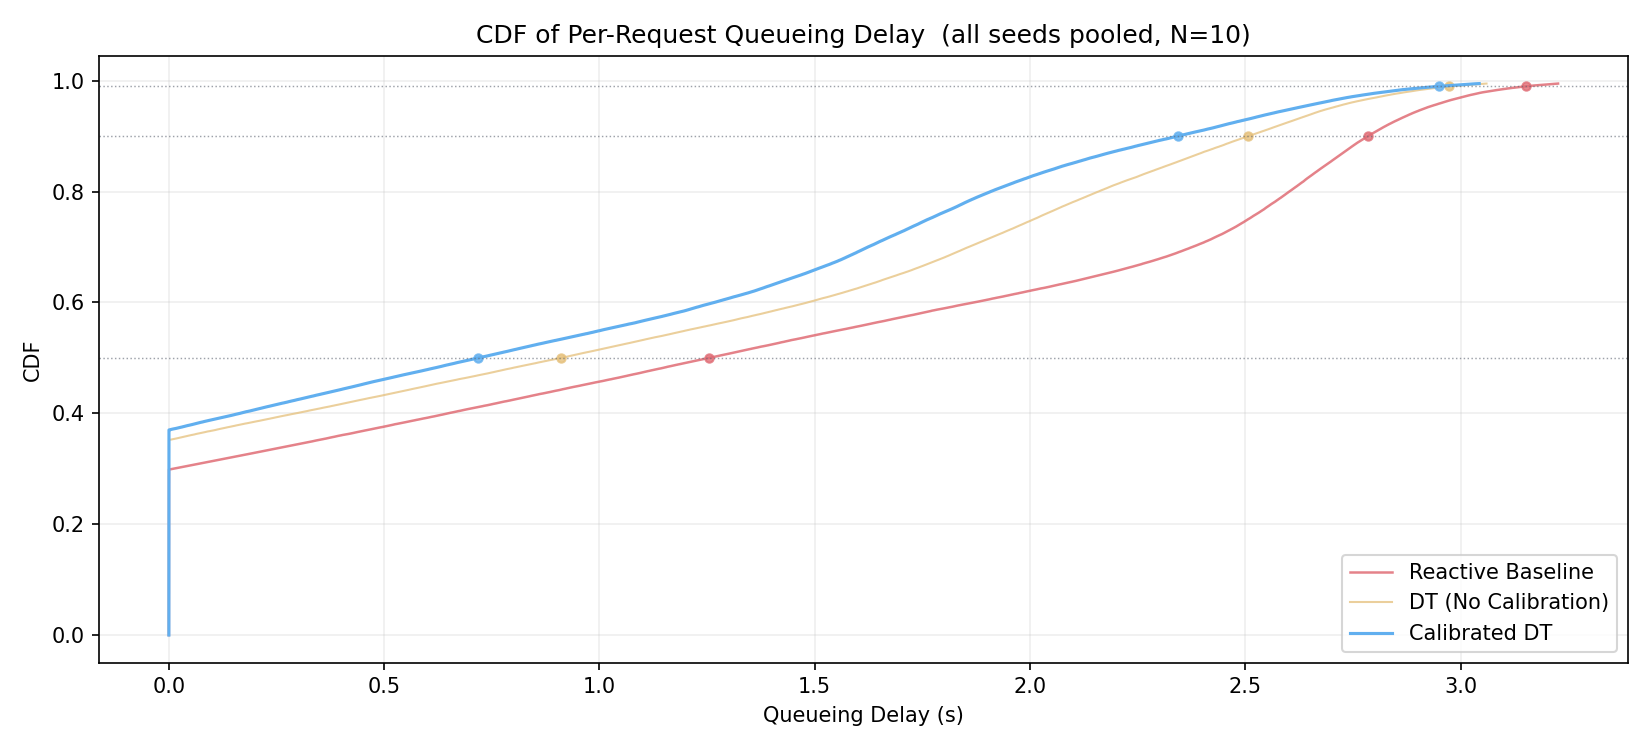
\includegraphics[width=\columnwidth]{phase5_delay_cdf.png}}
\caption{Per request queueing delay cumulative distribution function. All seeds are pooled. Filled markers denote the P50, P90, and P99 percentiles. The left shift of the Calibrated DT curve indicates a lower delay distribution.}
\label{fig:delay_cdf}
\end{figure}

The CDF of the calibrated DT is shifted left relative to both the reactive baseline and the uncalibrated DT. The reactive baseline allows requests entering the waiting queue near saturation to experience prolonged delays, which appears as large jumps in the P90 and P99 queueing delay values. Since the calibrated DT keeps $\qreal$ in a stable operating region, it suppresses the tail of the delay distribution. Compared to the uncalibrated DT, the calibrated DT reduces dropped connections; compared to the reactive baseline, it achieves statistically equivalent connection success while lowering queueing delay for served requests.

\subsection{Epsilon Sensitivity Analysis}

An exploratory sensitivity analysis over $\varepsilon \in \{5, 10, 20, 40, 80\}$ was conducted with a single random seed (seed 42). In this run, $\varepsilon = 40$ achieved the highest composite objective score, while $\varepsilon = 80$ produced the lowest mean state mirroring error. The selected value $\varepsilon = 10$ should therefore be interpreted as a conservative operating default motivated by the normal traffic noise floor rather than as a statistically validated optimum. A full multi seed sensitivity sweep is left for future work.

\subsection{Computational Complexity Analysis}

Integrating the calibrated DT controller into real gNB hardware requires minimal overhead. Each $\Delta$ step in Algorithm 1 involves a fixed number of arithmetic operations: one division, one multiply-add pair, one clip, and a few comparisons. Stored state is limited to $\{\ema_t, \qvirt, \alpha, n_{\mathrm{win}}\}$. The controller therefore requires $O(1)$ time and $O(1)$ space per control step, which suits the constrained resources of gNB hardware.

This contrasts with learning-based proactive controllers. In Machine Learning (ML) and Deep Neural Network (DNN) based approaches, inference cost scales with the size of the network weight matrix and reaches $O(W)$, where $W$ denotes the number of trained weights and therefore model capacity. Traffic predictors based on LSTM and Transformer models commonly reach $W \sim 10^5$--$10^7$, and inference latency at that scale can be on the order of milliseconds and may be non deterministic~\cite{b9}. In contrast, the real time response requirements of gNB RACH controllers are in the microsecond range. Deploying DNN based controllers directly on embedded hardware is therefore impractical from both latency and determinism perspectives.

The proposed $O(1)$ calibrated DT architecture addresses this tradeoff by providing online adaptation with minimal algorithmic overhead. Because each $\Delta = 1\ \mathrm{s}$ step consists only of fixed cost arithmetic and comparisons, the controller is suitable for implementation within commercial gNB software stacks, subject to target hardware benchmarking.

\subsection{O-RAN Integration and Real Time Deployment}

The calibrated DT controller maps directly onto the Open Radio Access Network (O-RAN) architecture. In the layered reference architecture defined by the O-RAN Alliance, the \emph{Near Real Time RAN Intelligent Controller} (Near-RT RIC) manages control loops between 10 ms and 1 s~\cite{b14}. The control interval $\Delta = 1\ \mathrm{s}$ used here matches the upper end of that range, while the $O(1)$ computational complexity indicates that the controller is a plausible candidate for tighter timing budgets after implementation-level latency validation.

In deployment, the calibrated DT controller is implemented as an \emph{xApp} running on the Near-RT RIC. The xApp receives input through the \textbf{E2} interface, where the gNB reports cell level RACH metrics such as $\qreal$, preamble collision count, and the per window arrival count $n_{\mathrm{win}}$ within the E2SM-KPM framework. The xApp executes Algorithm 1 and outputs the computed $\pacb$.

The generated $\pacb$ is then delivered to the gNB CU-CP through the \textbf{E2SM-RC} interface. The CU-CP injects this value into the uac-BarringInfo field of the SIB1 broadcast, fully consistent with the 5G NR Unified Access Control framework discussed earlier. The entire control loop thus closes over standard O-RAN and 3GPP signaling infrastructure without requiring protocol modifications or special hardware.

This deployment model has two practical advantages. First, operator policy intent, such as attack sensitivity level or the threshold $\varepsilon$, can be updated dynamically at xApp runtime through the Non-RT RIC. Second, the xApp abstraction provides a vendor independent deployment path, allowing the same controller to run across hardware from different vendors.

% =============================================================================
% SECTION 6: DISCUSSION AND LIMITATIONS
% =============================================================================
\section{Discussion and Limitations}

The calibrated DT architecture reduces state mirroring error and suppresses queueing delay tails in the modeled single-cell scenario. These results rest on simplifying assumptions that bound their generalizability.

\textbf{Single Cell Scope.} The adopted $MMPP/M/c/K$ model treats a single gNB cell independently. In real 5G deployments, there are continuous handover signaling flows between neighboring cells, mobility dependent correlations across UEs, and multi cell interference effects. These factors complicate the observation process of $\qreal$ in ways that cannot be fully represented by independent Markov chains. As a result, the 42\% reduction in state mirroring error observed in a single cell environment may differ in a multi cell deployment. Addressing this limitation would require either one DT instance per cell or a distributed architecture in which inter cell state sharing is coordinated centrally.

\textbf{Fixed Calibration Steps.} The proposed asymmetric calibration rule relies on fixed step sizes $\delta^{+} = 0.05$ and $\delta^{-} = 0.01$. These values were chosen through intuitive justification and practical bounds, while the $\varepsilon$ sensitivity analysis remains exploratory because it was performed with a single seed. Keeping $\delta^{+}$ and $\delta^{-}$ fixed creates a potential vulnerability: slow ramp attacks that deliberately keep botnet traffic just below the threshold $\varepsilon$ could push $\qreal$ gradually toward $K$ without ever triggering the calibration loop. This reveals a limitation against more sophisticated attacks. A natural next step is to determine $\delta^{+}$ and $\delta^{-}$ dynamically using a Reinforcement Learning (RL) agent that treats instantaneous state mirroring error as a reward signal.

% =============================================================================
% SECTION 7: CONCLUSION
% =============================================================================
\section{Conclusion}

This paper proposed and evaluated a calibrated Digital Twin architecture that proactively counters botnet-driven RRC signaling storm attacks on the 5G NR gNB RACH. Current reactive ACB mechanisms are inadequate under sudden burst conditions because of control loop latency, and standard proactive DT approaches accumulate state mirroring error under non-stationary traffic transitions.

The proposed system measures the state mirroring error $E = |\qreal - \qvirt|$ at every control step with $\Delta = 1\ \mathrm{s}$ and updates the EMA weight autonomously through the asymmetric calibration rule in Eq.~\eqref{eq:calibration}. Simulation results validated over $N=10$ independent seeds show that the calibration loop reduces state mirroring error by 42\%, suppresses the tail of the queueing delay distribution, and preserves the connection success rate at a level statistically equivalent to the reactive baseline.

Proactive control in non-stationary 5G environments requires both a sound control policy and tight alignment between the virtual model and the physical system. Suppressing state mirroring error is therefore a necessary condition for deploying DT-based proactive controllers in practice.

Two directions remain open. First, the architecture should be extended to multi-cell environments. Second, the fixed step sizes $\delta^{+}$ and $\delta^{-}$ should be learned dynamically through a Reinforcement Learning (RL) agent that uses state mirroring error as a reward signal.

% =============================================================================
% REFERENCES
% =============================================================================
\begin{thebibliography}{00}

\bibitem{b1}
A. Tabiban, H. A. Alameddine, M. A. Salahuddin, and R. Boutaba,
``Signaling Storm in O-RAN: Challenges and Research Opportunities,''
\emph{IEEE Commun. Mag.},
vol.~62, no.~6, pp.~58--64, Jun. 2024.

\bibitem{b2}
B. H. Lee, H. S. Lee, S. Moon, and J. W. Lee,
``Enhanced Random Access for Massive-Machine-Type Communications,''
\emph{IEEE Internet of Things J.},
vol.~8, no.~8, pp.~7046--7064, Apr. 2021.

\bibitem{b3}
M. Grieves and J. Vickers,
``Digital Twin: Mitigating Unpredictable, Undesirable Emergent Behavior in
Complex Systems,''
\emph{Transdisciplinary Perspectives on Complex Systems},
F.-J. Kahlen, S. Flumerfelt, and A. Alves, Eds.
Cham: Springer, 2017, pp.~85--113.

\bibitem{b4}
3rd Generation Partnership Project (3GPP),
``NR; Radio Resource Control (RRC) Protocol Specification,''
TS~38.331, version~17.3.0, Release~17, Jan. 2023.

\bibitem{b5}
L. Miuccio, D. Panno, and S. Riolo,
``Joint Control of Random Access and Dynamic Uplink Resource Dimensioning
for Massive MTC in 5G NR Based on SCMA,''
\emph{IEEE Internet of Things J.},
vol.~7, no.~6, pp.~5042--5063, Jun. 2020.

\bibitem{b6}
J.-B. Seo, W. T. Toor, and H. Jin,
``Analysis of Two-Step Random Access Procedure for Cellular Ultra-Reliable Low Latency Communications,''
\emph{IEEE Access},
vol.~9, pp.~5972--5985, Jan. 2021.

\bibitem{b7}
S. K. Sharma and X. Wang,
``Toward Massive Machine Type Communications in Ultra-Dense Cellular IoT
Networks: Current Issues and Machine Learning-Assisted Solutions,''
\emph{IEEE Commun. Surveys Tuts.},
vol.~22, no.~1, pp.~426--471, 1st Qtr. 2020.

\bibitem{b8}
R. Dong, C. She, W. Hardjawana, Y. Li, and B. Vucetic,
``Deep Learning for Radio Resource Allocation With Diverse Quality-of-Service
Requirements in 5G,''
\emph{IEEE Trans. Wireless Commun.},
vol.~20, no.~4, pp.~2309--2324, Apr. 2021.

\bibitem{b9}
C. Zhang, P. Patras, and H. Haddadi,
``Deep Learning in Mobile and Wireless Networking: A Survey,''
\emph{IEEE Commun. Surveys Tuts.},
vol.~21, no.~3, pp.~2224--2287, 3rd Qtr. 2019.

\bibitem{b10}
H. X. Nguyen, R. Trestian, D. To, and M. Tatipamula,
``Digital Twin for 5G and Beyond,''
\emph{IEEE Commun. Mag.},
vol.~59, no.~2, pp.~10--15, Feb. 2021.

\bibitem{b11}
P. Almasan, M. Ferriol-Galmes, J. Paillisse, J. Suarez-Varela,
D. Perino, D. Lopez, A. A. Pastor Perales, P. Harvey, L. Ciavaglia,
L. Wong, V. Ram, S. Xiao, X. Shi, X. Cheng, A. Cabellos-Aparicio,
and P. Barlet-Ros,
``Network Digital Twin: Context, Enabling Technologies, and Opportunities,''
\emph{IEEE Commun. Mag.},
vol.~60, no.~11, pp.~22--27, Nov. 2022.

\bibitem{b12}
R. F. Olimid and G. Nencioni,
``5G Network Slicing: A Security Overview,''
\emph{IEEE Access},
vol.~8, pp.~99999--100009, Jun. 2020.

\bibitem{b13}
Q. Xu, S. Ali, and T. Yue,
``Digital Twin-Based Anomaly Detection in Cyber-Physical Systems,''
\emph{Proc. IEEE Conf. Software Testing, Verification and Validation (ICST)},
Porto de Galinhas, Brazil, Apr. 2021, pp.~205--216.

\bibitem{b14}
M. Polese, L. Bonati, S. D'Oro, S. Basagni, and T. Melodia,
``Understanding O-RAN: Architecture, Interfaces, Algorithms, Security,
and Research Challenges,''
\emph{IEEE Commun. Surveys Tuts.},
vol.~25, no.~2, pp.~1376--1411, 2nd Qtr. 2023.

\end{thebibliography}

\end{document}
